\PassOptionsToPackage{hyphens}{url}
\documentclass[compress,aspectratio=169]{beamer}

\usetheme{Reading}

\graphicspath{{../2019-06-isc/}{../2019-06-isc/fig/}{img/}{../logo/}}

\newcommand{\ok}[1]{{#1 (done)}}
\newcommand{\ongoing}[1]{{#1 (ongoing)}}
\newcommand{\started}[1]{{#1 (started)}}
\newcommand{\pending}[1]{{#1 (pending in plan)}}
\newcommand{\hrefb}[2]{\href{#1}{\textcolor{red}{#2}}}

\subtitle{}
\title{\Large The HPC Certification Forum -- Activity Update 2020}
\author{Julian Kunkel (+ HPC Certification Forum)}
\date{2020-05-20}
\authorURL{https://hpc-certification.org}
\authorFooter{Julian M. Kunkel et al.}
\venue{HETET20 Workshop}
\institute{Department of Computer Science}
\groupLogo{
\includegraphics[width=2.5cm]{hpccf-small}}
\titleLogo{ 
\includegraphics[height=2.5cm]{blur-book-stack-books-590493}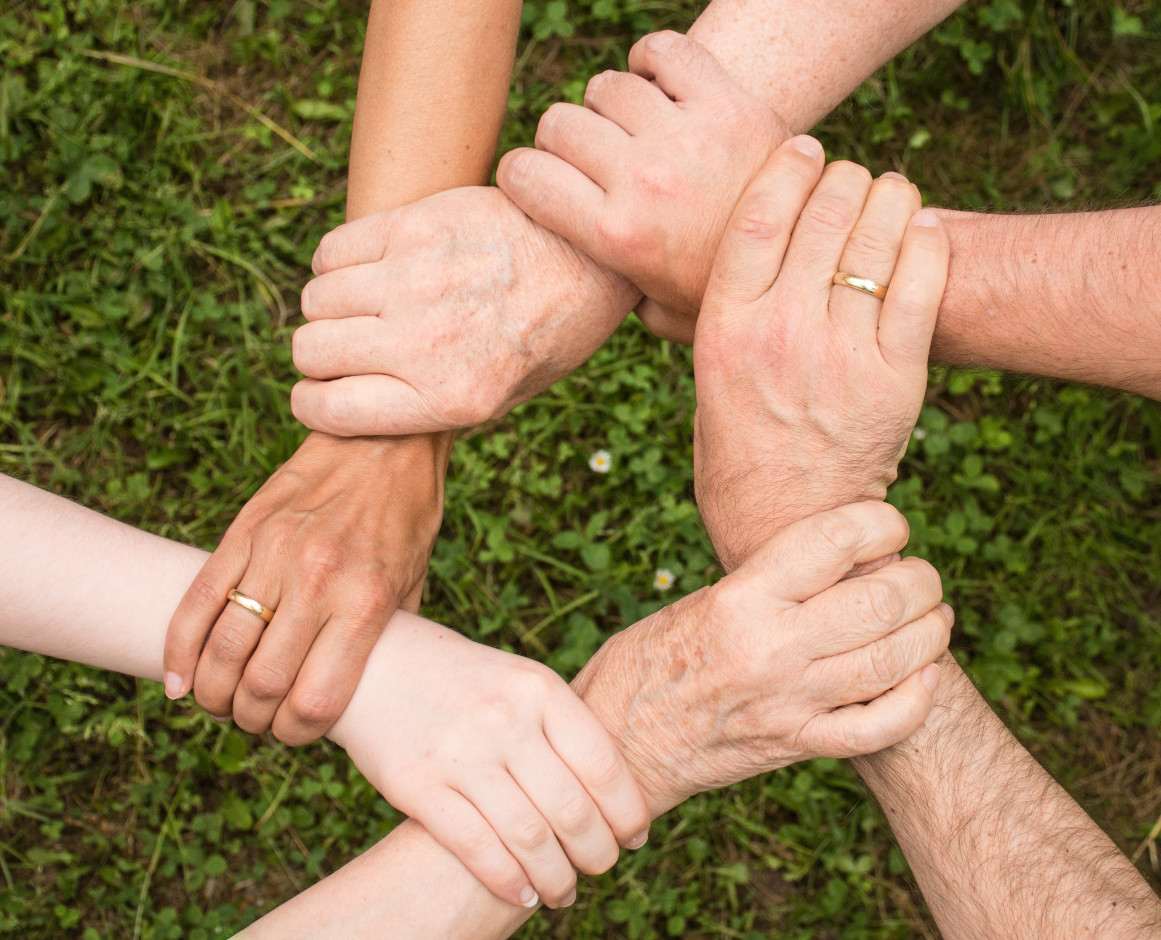
\includegraphics[height=2.5cm]{ground-group-growth-461049}
\includegraphics[height=2.5cm]{accomplishment-ceremony-college-267885}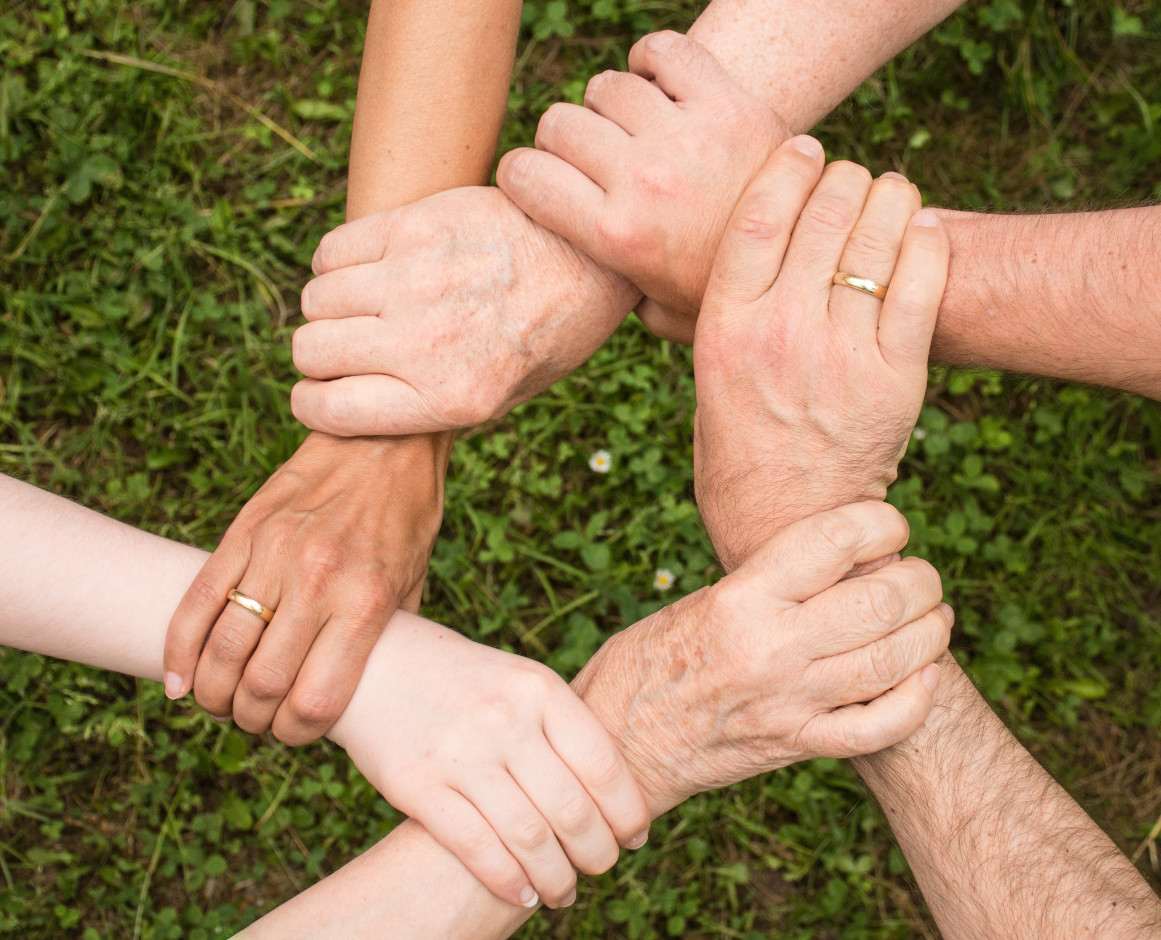
\includegraphics[height=2.5cm]{ground-group-growth-461049}
\includegraphics[height=2.5cm]{blur-book-stack-books-2}}


\begin{document}

\begin{frame}[plain]{}
	\maketitle
\end{frame}


%       the nature of the training or education program
%       Strategy
%       assessment or evaluation technique
%       situations for which it is relevant or in which it was applied
%       an evaluation of its success
%       lessons learned
%       reproducibility of the processes and resources


\section{The Forum}
\subsection{}



\begin{frame}{The 
\includegraphics[width=0.45\textwidth]{hpccf-full}}
		\begin{block}{Goals}
			\begin{itemize}
				\item Fine-grained standardizing HPC knowledge representation
          \begin{itemize}
            \item What competences exist, how are they defined?
            \item Puzzle of competences for everyone (practitioners, students, admins)
            \item Supporting navigation and role-specific knowledge maps
          \end{itemize}
				\item Establishing international certificates attesting knowledge
        \item Supporting an ecosystem around the HPC competences
			\end{itemize}
		\end{block}

    \begin{block}{Scope of the forum}
    \begin{itemize}
      \item Central authority for competence representation, certification, and support
      \item Purposeful limitations of the forum:
			\begin{itemize}
				\item We do not compete with content providers (we do link their content though)
				\item We do not create a curriculum (university/centers responsibility)
			\end{itemize}
    \end{itemize}
		\end{block}
\end{frame}


\begin{frame}{The 
\includegraphics[width=0.45\textwidth]{hpccf-full}}

	\begin{block}{Organization Details}
		\begin{itemize}
			\item An independent international body
			\item Organized into
				\begin{itemize}
					\item Steering board (elected)
					\item Full members (with voting rights)
            \begin{itemize}
              \item Contributors to the project (e.g., 1-2 hours per month)
            \end{itemize}
					\item Associate members (anyone and any institution)
          \item Collaboration with e.g., SIGHPC Education Chapter
				\end{itemize}
		\end{itemize}
	\end{block}

	\begin{block}{Responsibilities}
		\begin{itemize}
			\item Curating and maintaining the skill tree and certificates
			\item Providing tools and ecosystem around the competences
		\end{itemize}
	\end{block}
\end{frame}


\begin{frame}{Organization}
  \begin{block}{Organization of the members}
	\begin{itemize}
  \item Webpage is the central hub (\url{https://www.hpc-certification.org})
  \item Mailinglists (news, members, board)
	\item Monthly public meetings on our Slack channel
  \item Annual general assembly (form of a BoF at ISC or workshop)
  \end{itemize}
  \end{block}

  \begin{block}{Data handling}
    \begin{itemize}
      \item Everything* is developed/available in the open \\
        GitHub (\url{https://github.com/HPC-certification-forum})
      \item Exception are examination questions (later talk)
    \end{itemize}
  \end{block}
\end{frame}


\section{Skills}
\sectionIntroHidden

\begin{frame}{Classification of Competences == Skills}
	\begin{itemize}
		\item A \textbf{skill} defines background, objectives, learning outcomes
		\item The \textbf{skill tree} organizes the competences as hierarchical skills
		\item Certificates bundle several skills into attestable unit
	\end{itemize}

	\begin{figure}
		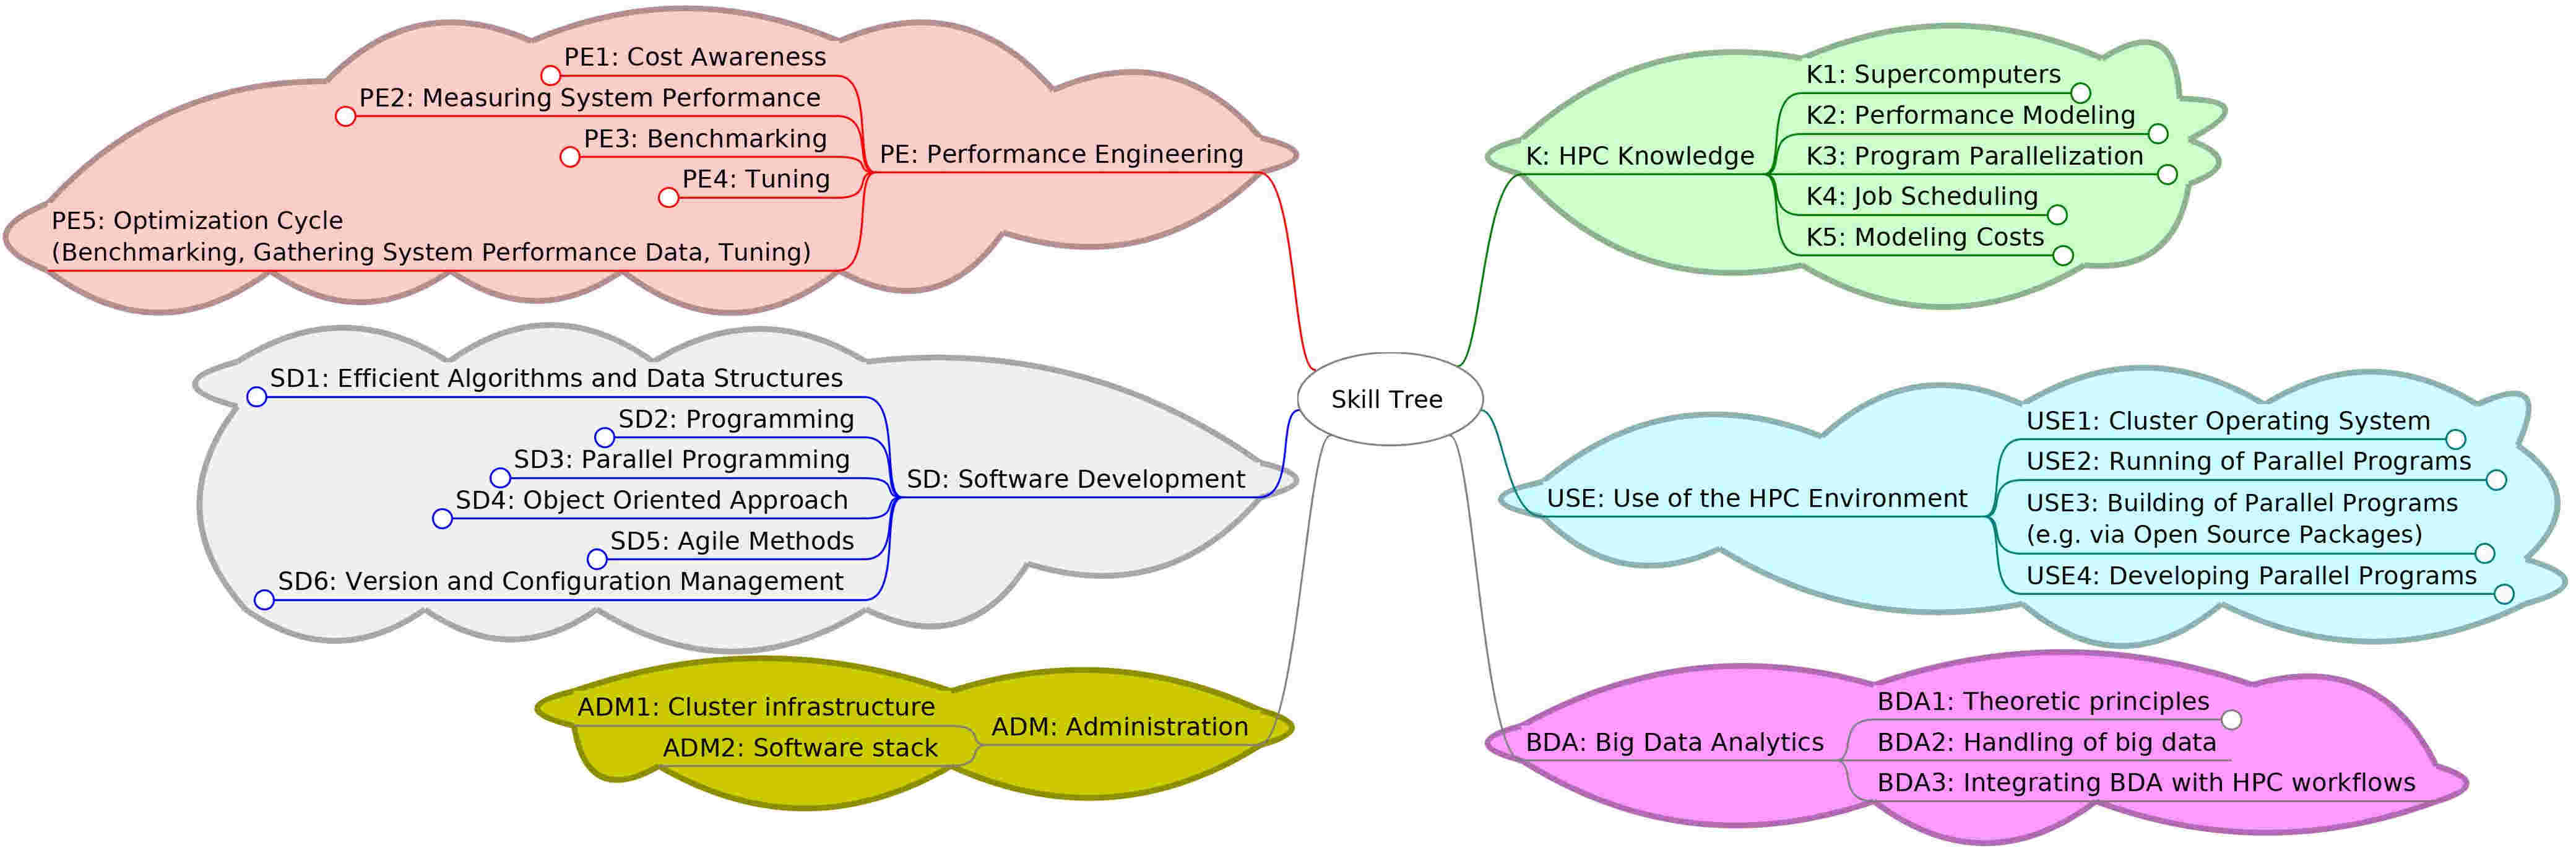
\includegraphics[width=\textwidth]{skill-tree}
		\vspace*{-2em}
		\caption{Top-levels of the skill tree (Initial ADM and BDA branches)}
	\end{figure}
\end{frame}


\begin{frame}{Example High-Level Skill (Excerpt)}
\begin{itemize}
\item Name: SLURM Workload manager
\item Id: USE4.2.2-B
\item Background: {\small SLURM is a widely used open-source workload
manager providing various advanced features.}
\item Aim:
\begin{itemize}
\item comprehend and describe the basic architecture of SLURM and its tools
\item use relevant tools to run and monitor (parallel) applications
\end{itemize}
\end{itemize}

\begin{block}{Learning outcomes (these must be examinable)}
\begin{itemize}
\item run interactive jobs with salloc, a batch job with sbatch
\item explain the architecture of SLURM, i.e., the role of slurmd, srun
\item explain the function of the tools: sacct, sbatch, salloc, ...
\item explain time limits and the benefit of a backfill scheduler
\item \textit{see \url{https://www.hpc-certification.org/wiki/}}
\end{itemize}
\end{block}
\end{frame}



\section{Status and Outlook}
\sectionIntroHidden


\begin{frame}{Status}

  \begin{itemize}
    \item We have been working on processes, tools, content (\hrefb{https://www.hpc-certification.org/}{webpage})
  \end{itemize}


\begin{block}{Processes}
  \begin{itemize}
    \item Contribution of content (skills, exam questions)
    \item Examination/Certification process
    \item Versioning of the skill tree
    \item Endorsment of training material
    \item Governance rules (coarse grained)
    \item Roadmap development
  \end{itemize}
\end{block}


\begin{block}{Content}
	\begin{itemize}
	\item A subtree of the skill tree is considered ready for release
  \item Created small set of demo content for tools/processes
  \end{itemize}
\end{block}
%\textit{All our developments are under open licenses (except the exam questions)}
\end{frame}

\begin{frame}{Status}

\begin{block}{Tools (prototypes exist)}
  \begin{itemize}
    \item Markdown version of skill definition
      \begin{itemize}
        \item Version controlled on GitHub
        \item Synchronized with a (Doku)Wiki for simple access
        \item Tool for synchronization with FreePlane MindMap
      \end{itemize}
    \item JavaScript for user-visualized skill tree \hrefb{https://www.hpc-certification.org/skills/}{(demo)}
  		\begin{itemize}
  			\item Adjustable/embedable in your webpage, blend in your data to the skill tree
        \item Example, add links to own material, show relevant skills to users
      \end{itemize}
    \item Online test execution
      \begin{itemize}
        \item Registration till certificate
        \item Exam itself: multiple choice, other question types will follow
      \end{itemize}
    \item RESTful service to query information about skills
      \begin{itemize}
        \item Allow to add supplementary information such as existing teaching material
      \end{itemize}
  \end{itemize}
\end{block}

\end{frame}


\begin{frame}{Summary}

	\begin{block}{HPC Certification Program}
		\begin{itemize}
			\item Effort to standardize representation/certification of relevant HPC skills
      \begin{itemize}
        \item Hierarchical definition of skills for practitioners
        \item Building blocks that can be cherry-picked for different tasks
				\item It's goal is \textbf{NOT} to provide content or a linear curriculum
      \end{itemize}
      \item We are on track with the effort but need support of the community
      \item Visit us and join our Slack/mailing lists: \url{https://hpc-certification.org}
		\end{itemize}
	\end{block}
\end{frame}




\end{document}
